\documentclass[a4paper, 12pt]{article}

\usepackage{hyperref}
\usepackage[warn]{mathtext}
\usepackage[utf8]{inputenc}
\usepackage[T2A]{fontenc}
\usepackage[english,russian]{babel}
\usepackage{multirow}
\usepackage{float}
\restylefloat{table}
\usepackage{amsmath,amsfonts,amssymb,amsthm,mathtools}
\usepackage{indentfirst}
\DeclareSymbolFont{T2Aletters}{T2A}{cmr}{m}{it}
\usepackage{ gensymb }
\mathtoolsset{showonlyrefs=true}
\usepackage{euscript}
\usepackage{mathrsfs}
\usepackage[left=2cm,right=2cm,top=2cm,bottom=2cm]{geometry}
\usepackage{graphicx}
\usepackage{wrapfig}
\usepackage[rgb]{xcolor}
\hypersetup{
colorlinks=true,
urlcolor=blue
}
\usepackage{tikz}

\title{Лабораторная работа}
\author{Гисич Арсений Б03-101}
\date{2023}

\begin{document}

	\begin{center}
		{\large МОСКОВСКИЙ ФИЗИКО-ТЕХНИЧЕСКИЙ ИНСТИТУТ (НАЦИОНАЛЬНЫЙ ИССЛЕДОВАТЕЛЬСКИЙ УНИВЕРСИТЕТ)}
	\end{center}
	\vspace{5 cm}
	{\Large
		\begin{center}
			{\bf Лабораторная работа 5.4.1}\\[0.2 cm]
			Определение энергии $\alpha$-частиц по величине их пробега в воздухе
		\end{center}
	}
	\vspace{4 cm}
	\begin{flushright}
		{\Large Выполнили: \\
			\vspace{0.2 cm}
			Гисич Арсений \\
            Вазюля Василиса \\ 
			\vspace{0.2 cm}
			Б03-101 \\}
	\end{flushright}
	\vspace{8 cm}
	\begin{center}
		Долгопрудный\\[0.1 cm]
		2023
	\end{center}
\thispagestyle{empty}

\section{Аннотация}

В данной работе измерялся пробег альфа-частиц в воздухе двумя способами: с помощью торцевого счетчика Гейгера и ионизационной камеры.

\section{Теоретические сведения и методика измерений}

В качестве источника альфа-частиц используется $ ^{239}  $Pu  с периодом полураспада $ T_{1/2} = 2,44 \times 10^4 $ лет. Альфа-частицы, испускаемые $ ^{239} Pu $, состоят из трех моноэнергетических групп, различие между которыми лежит в пределах 50 кэВ. При той точности, которая достигается
	в наших опытах, их можно считать совпадающими по энергии, равной
	5,15 МэВ.
	
	\subsection{Счетчик Гейгера}
	
	\begin{wrapfigure}[17]{l}{0.25\linewidth}
		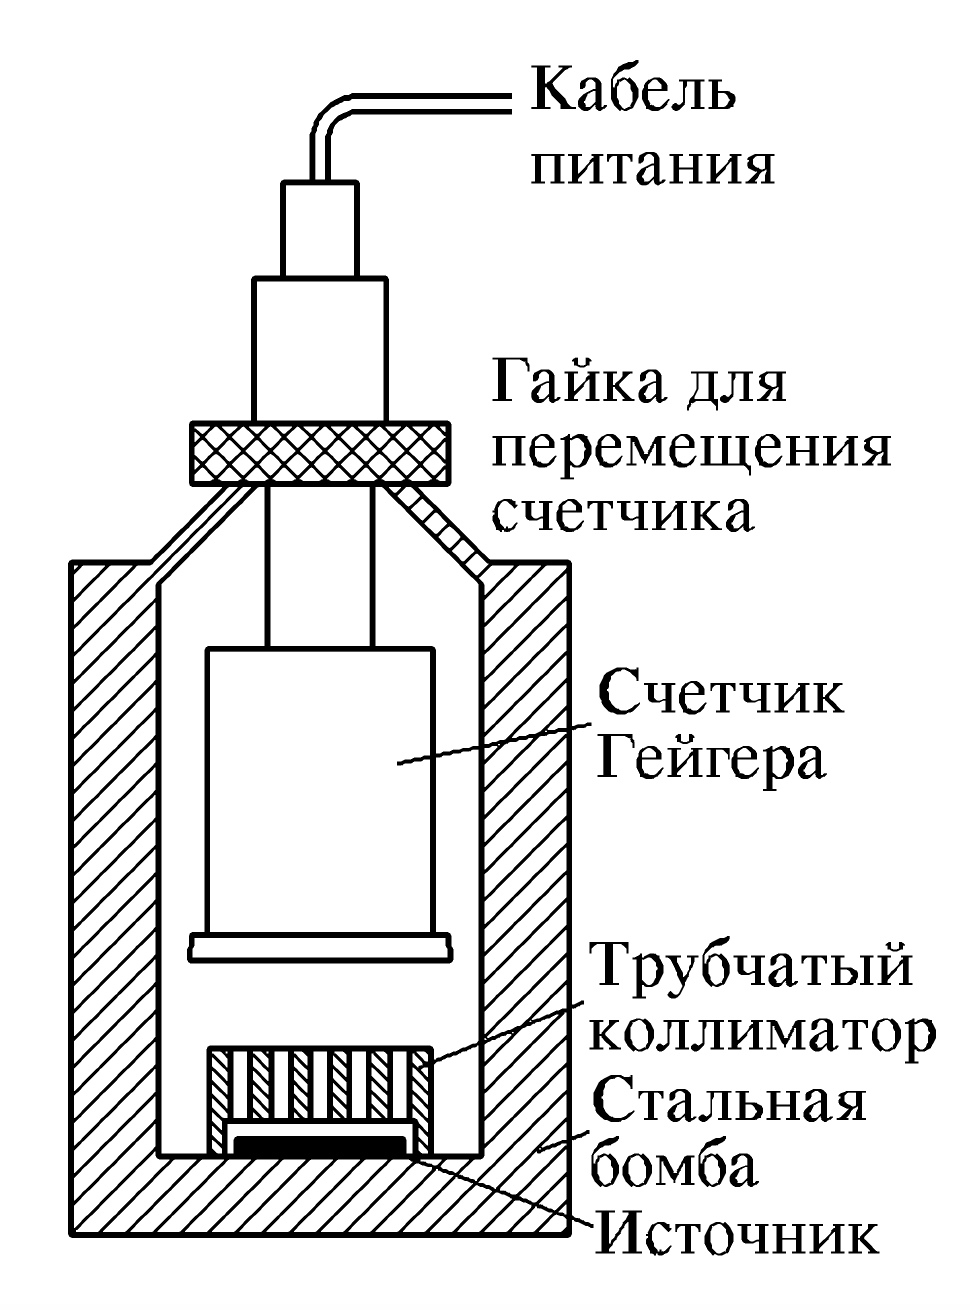
\includegraphics[width=\linewidth]{Geyger}
		\caption{Схема торцевого счетчика Гейгера}
		\label{ris geyger}
	\end{wrapfigure}
	
	Для определения пробега альфа-частиц с помощью счетчика радиоактивный источник помещается на дно стальной цилиндрической бомбы
	(рис. \ref{ris geyger}), в которой может перемещаться торцевой счетчик Гейгера. Его
	чувствительный объем отделен от наружной среды тонким слюдяным
	окошком, сквозь которое могут проходить альфа-частицы. Рабочее напряжение счетчика указано на установке.
	
	Импульсы, возникающие в счетчике, усиливаются и регистрируются пересчетной схемой. Путь частиц в воздухе зависит от расстояния между источником и счетчиком. Перемещение счетчика производится путем вращения гайки, находящейся на крышке бомбы. Расстояние
	между счетчиком и препаратом измеряется по шкале, нанесенной на
	держатель счетчика. Счетчик не может быть придвинут к препарату ближе чем на 10 мм, т. к. между источником и счетчиком установлен коллиматор, изготовленный из плотно сжатых металлических трубок. Отверстия трубок пропускают к счетчику только те альфа-частицы, которые вылетают из источника почти перпендикулярно его поверхности.
	
	\subsection{Ионизационная камера}
	
	Ионизационная камера --- прибор для количественного измерения
	ионизации, произведенной заряженными частицами при прохождении
	через газ. Камера представляет собой наполненный газом сосуд с двумя электродами (схема камеры приведена на рис. \ref{ris Ion}). Сферическая стенка прибора служит одним из электродов, второй электрод вводится в газ через изолирующую пробку. К электродам подводится постоянное напряжение от источника ЭДС.
	
	Заполняющий сосуд газ сам по себе не проводит электрический ток, возникает он только при прохождении быстрой заряженной частицы, которая рождает в газе на своем пути ионы.
	
	Поместим на торец внутреннего электрода источник
	ионизирующего излучения (в нашем случае это источник
	альфа-частиц $ ^{239}_{94} $Pu), заполним объем камеры воздухом и начнем
	постепенно увеличивать разность потенциалов между электродами. Ток, протекающий через камеру, вначале будет резко возрастать, а затем, начиная с некоторого напряжения $ V_0 $, станет постоянным, т. е. "<выйдет на плато">.  Предельный ток $ I_0 $ будет равен $ I_0 = n_0e $,
	где $ n_0 $ --- число пар ионов, образуемых в секунду в объеме камеры, а $ e $ --- заряд электрона.
	
	\begin{wrapfigure}[17]{l}{0.37\linewidth}
		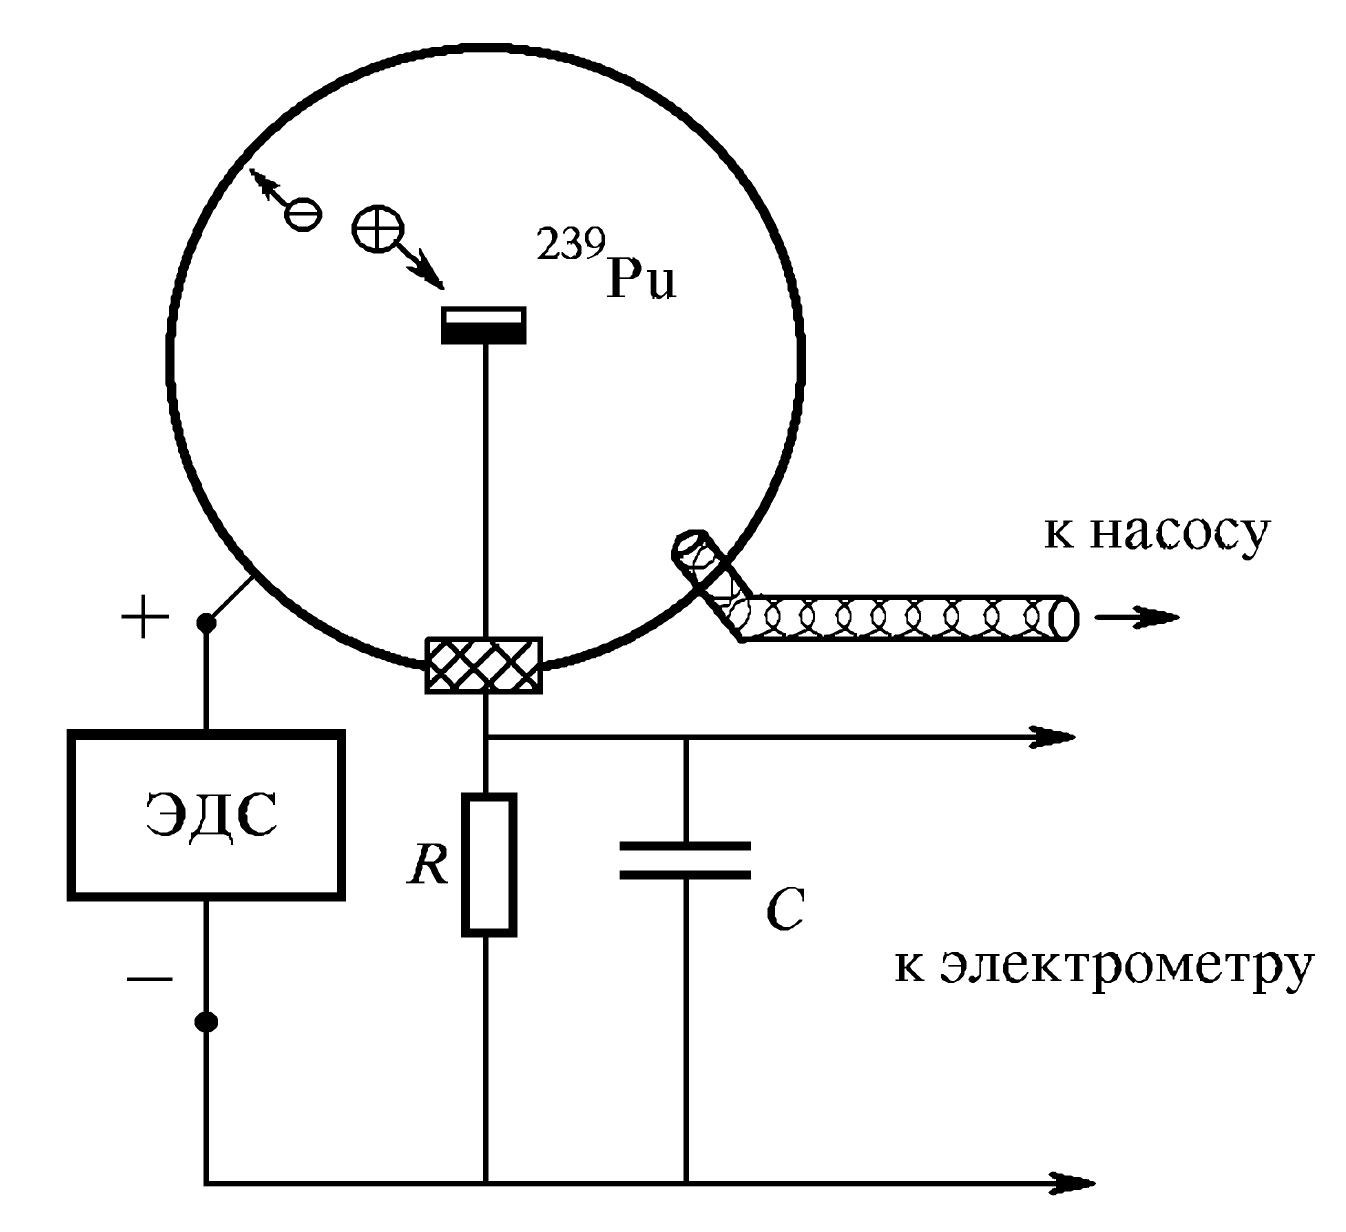
\includegraphics[width=\linewidth]{Ion}
		\caption{Схема устройства ионизационной камера}
		\label{ris Ion}
	\end{wrapfigure}
	
	Прохождение тока через камеру регистрируется посредством измерения напряжения на включенном в цепь камеры сопротивлении $ R $.
	Так как средняя энергия ионизации атомов воздуха составляет около 30 эВ, то альфа-частица с энергией 3 МэВ образует на своем пути около $ 10^5 $ электронов, им соответствует заряд $1,6 \times 10^{-14} $ Кл. Чтобы
	столь малое количество заряда, создаваемое проходящей через камеру одной альфа-частицей, вызывало измеряемое напряжение, емкость $ C $
	должна быть мала.
	
	Так как подвижность электронов примерно в 1000 раз больше подвижности ионов, то подбором параметров $ RC $-цепочки можно выделить импульсы тока, соответствующие только возникающей электронной компоненте. Реально регистрация электронной компоненты
	импульса тока обеспечивается при величине постоянной времени $ RC $-цепочки в несколько микросекунд.
	Если число проходящих через камеру альфа-частиц достаточно велико, то можно регистрировать не заряд, а величину возникающего тока, которая, естественно, пропорциональна интенсивности альфа-частиц. В
	токовом режиме величину постоянной времени $ RC $-цепочки устанавливают равной нескольким секундам, а работающую в этом режиме
	камеру называют токовой.
	
	\begin{wrapfigure}[19]{r}{0.3\linewidth}
		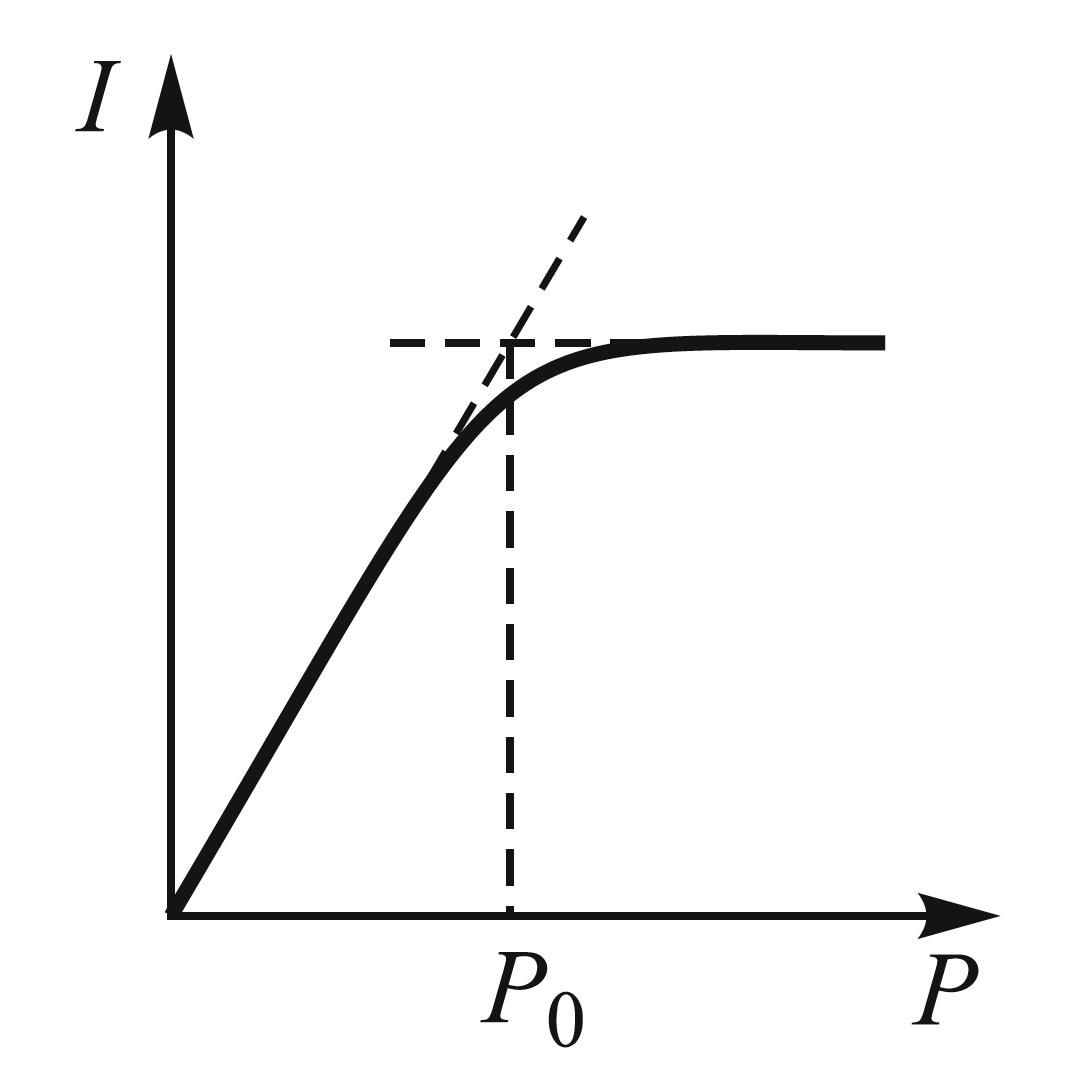
\includegraphics[width=\linewidth]{PotI}
		\caption{Характерная кривая зависимости
			тока ионизационной камеры от давления.
			Ионизация создается $ \alpha $-частицами}
		\label{ris PotI}
	\end{wrapfigure}
	
	При изменении давления в камере ионизационный ток меняется так, как это показано на рис. \ref{ris PotI}. При небольших давлениях газа
	альфа-частицы передают часть энергии стенкам камеры. По достижении
	давления $ P_0 $ все они заканчивают свой пробег внутри газа, и дальнейшее возрастание тока прекращается. Для определения давления $ P_0 $ чаще всего пользуются методом экстраполяции (полученная таким методом величина называется экстраполированным пробегом), продолжая наклонный и горизонтальный участки кривой до пересечения. Найденный таким образом пробег затем должен быть приведен к нормальному давлению и температуре $ 15 ^\circ C $.
	
	В данной работе измерение пробега альфа-частицы проводится по величине тока ионизации в сферической камере. Внутренним электродом
	камеры служит диск диаметром 5 мм, на который нанесен тонкий слой $ ^{239}_{94} $Pu, покрытый сверху тонкой защитной пленкой. Вторым электродом служит внешняя оболочка камеры --- полый шар с внутренним
	диаметром 100 мм. Оба электрода тщательно изолированы один от
	другого и от земли. Разность потенциалов между электродами составляет 300 В. Вакуумная установка содержит кран и манометр. Она позволяет изменять давление в камере от атмосферного до 10 мм рт. ст.
	Величина тока ионизации измеряется электрометром, состоящим из
	нескольких стандартных микросхем, по величине падения напряжения
	на сопротивлении $ R $ = 100 МОм ($ C = 10^{-8} $ Фарад, так что $ RC $ = 1 с).
	Значение измеряемого ионизационного тока (в пикоамперах) высвечивается на цифровом табло.

\section{Результаты измерений и обработка данных}

\subsection{Исследование пробега с помощью счётчика Гейгера}

Проведём измерения зависимости скорости счёта $N$ от расстояния $x$ между источником и счётчиком. Результаты измерений представлены на графике рис.~\ref{plot:Geyger}. К значениям расстояния необходимо прибавить расстояние между счётчиком и коллиматором, равное 10~мм.

\begin{figure}[h]
\begin{center}
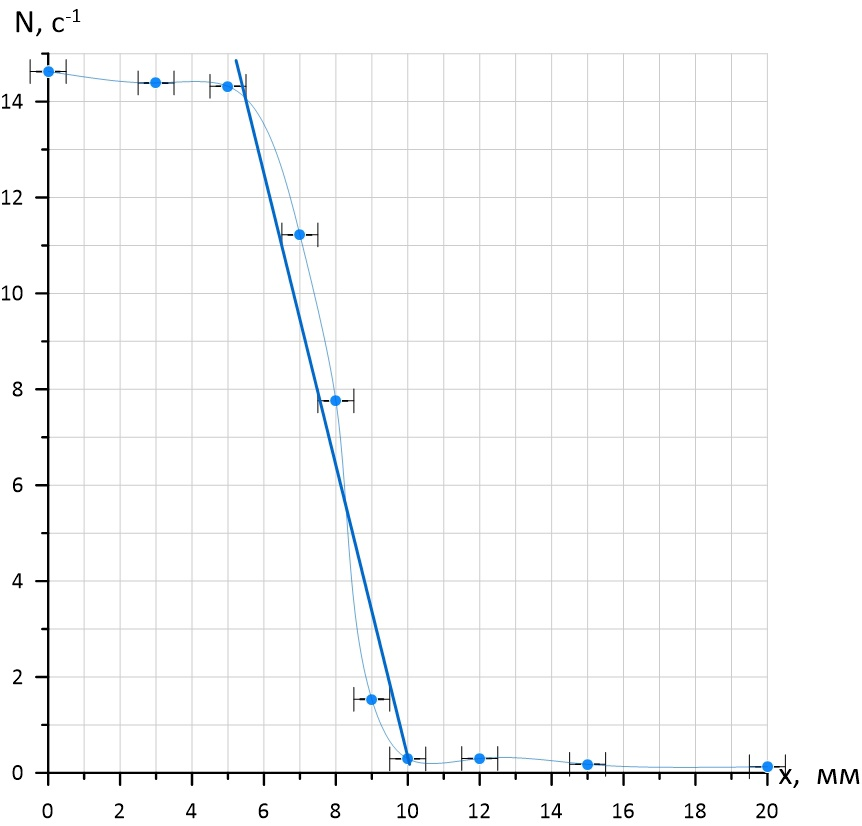
\includegraphics[width = 0.8\textwidth]{plotGeyger.jpg}
\caption{Зависимость $N = N(x)$}
\label{plot:Geyger}
\end{center}
\end{figure}

Экстраполируем полученную прямую до пересечения с осью абсцисс. Отсюда получаем экстраполированную длину пробега
		 
		 \begin{equation}\label{}
		 R_э = -\dfrac{b}{a} \approx 20,11 \pm 2,01 \; мм \Rightarrow R'_э = \rho R_э = (2,59 \pm 0,26)\cdot 10^{-3} \; г/см^2
		 \end{equation}
		
		Среднюю длину пробега оценим как $ R_{ср} \backsimeq 18,0 \pm 0,5 $ мм $ \Rightarrow R'_{ср} = \rho R_{ср} = (2,32 \pm 0,65)\cdot 10^{-3} \; г/см^2 $
		
		Энергию таких альфа-частицы можно оценить по эмпирической формуле 
		
		\begin{equation}\label{}
		R = 0,32 E^{3/2} \Rightarrow E_э \approx 3,41 \pm 0,23 \; МэВ, \quad E_{ср} \approx 3,16 \pm 0,21 \; МэВ
		\end{equation}
		
\subsection{Ионизационная камера}

Включив питание установки, измерим атмосферное давление $ P_а = 99,35 $~кПа (измеренно барометром). Температура $ T = 293 $ К. После этого откачаем воздух из камеры до давления порядка $ \backsimeq 10 $ Торр и снимем зависимость тока от давления. Результаты измерений представлены на рис.~\ref{plot:Ion}.

\begin{figure}[h]
\begin{center}
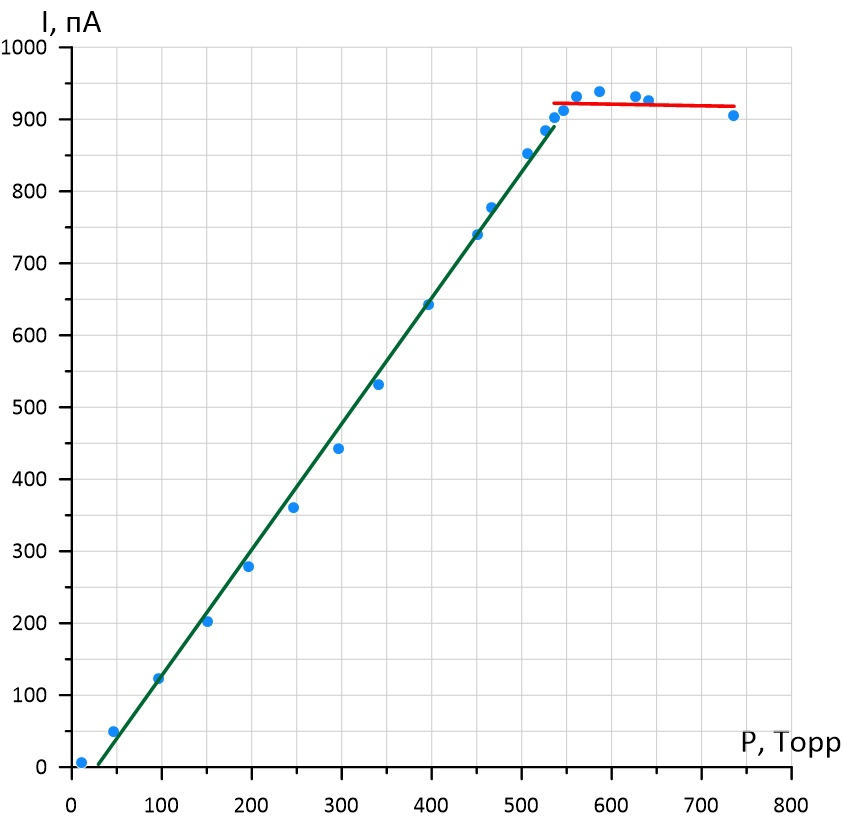
\includegraphics[width = 0.8\textwidth]{plotIon.jpg}
\caption{Зависимость $I = I(P)$}
\label{plot:Ion}
\end{center}
\end{figure}

График зелёной прямой:
$$ y = 1.75 \cdot x - 47.55$$
красной:
$$ y = -0.02 \cdot x + 934.35$$

Их пересечение дает нам значение 
	
	\begin{equation}\label{}
	P = \dfrac{b_2 - b_1}{a_1 - a_2} \approx (554 \pm 8) \; Торр 
	\end{equation}
	
	Так как пробег $ R_l = 5 $ см задается размером камеры, приведем его к н.у.:
	
	\begin{equation}\label{}
	R_э = R_l \dfrac{\rho}{\rho_0} = R_l \dfrac{P_0T}{PT_0} \approx (3,35 \pm 0,05) \; см \Rightarrow R'_э \approx (4,32 \pm 0,06)\cdot 10^{-3} \; г/см^2
	\end{equation}
	
	Энергию такой альфа-частицы можно оценить по эмпирической формуле 
	
	\begin{equation}\label{}
	R = 0,32 E^{3/2} \Rightarrow E_э = \left(  \dfrac{R_э}{0,32} \right)^{2/3} \approx 4,79 \pm 0,04 \; МэВ
	\end{equation}	

\section{Обсуждение результатов и выводы}

В данной работе был измерен пробег альфа-частиц от $ ^{239}  $Pu двумя способами: с помощью торцевого счетчика Гейгера и ионизационной камеры. По полученным данным была определена энергия альфа-частиц.
	
	При работе с ионизационной камерой пробег и энергия получились близкими к ожидаемым (из таблицы при $ E = 5 $ МэВ получаем $ R = 3,29 $ см для воздуха). При работе со счетчиком Гейгера значения пробега и энергий ниже табличных. Это можно объяснить тем, что часть энергии альфа-частиц тратится на прохождение слюдяной пластинки, прикрывающей счетчик, и пленки, закрывающей источник. 
	
	Если плотность бумаги равна $ 1,2 \; г/см^3 $, следовательно, лист бумаги толщины $~l~\geq~R'/\rho = 3,6 $~мкм не пропустит альфа-частицы от $ ^{239}  $Pu.

\end{document}
